\documentclass[10pt]{article}

\usepackage{amsmath}
\usepackage{amssymb}
\usepackage{booktabs}
\usepackage{graphicx}

\title{Disentangling Exemplar Replay in Class-Incremental Learning}
\author{}
\date{}

\begin{document}

\maketitle

\begin{abstract}
Replay-based class-incremental learning is specified by more than its memory
budget: exemplar selection, distillation, classifier geometry, and the final
readout can all affect retention.  We conduct a controlled study of these
choices on CIFAR-100 with ten class-incremental tasks, a ResNet-18 backbone,
and a fixed total exemplar budget.  Our reference rebuilds herded exemplars in
the current feature space after every task, trains with replay and old-class
distillation, and uses nearest-mean exemplar (NME) prediction.  At 2,000
exemplars and retrieval budget 64, it obtains $44.99\pm1.00\%$ final average
accuracy and $13.85\pm0.44\%$ forgetting.  Replacing NME with head-logit
evaluation reduces average accuracy by $10.38$ percentage points and increases
forgetting by $32.50$ points; replacing herding with random selection reduces
accuracy by $4.83$ points.  Removing distillation leaves average accuracy nearly
unchanged but increases forgetting by $10.93$ points.  Across the tested
resources, reducing memory from 2,000 to 500 exemplars has a larger effect on
accuracy than reducing retrieval from 64 to 32 samples.  These results identify
the readout, exemplar selection, and total memory as the principal design
choices in this protocol, while limiting the conclusion to the evaluated
dataset, class order, backbone, and budget range.
\end{abstract}

\section{Introduction}
\label{sec:introduction}

In the replay based incremental class learning, a small exemplar set represents whole training history. The backbone changes every new task, thus the exemplars selected under with old features no longer well approximate the class distributions during training. Current state of the art methods integrate selection, refresh timing, training objective, readout into one protocol, hence a performance gap between methods can not isolate the refresh rule with everything else in the method.

We propose Uniform Herding.  After each task is completed, it then divides the active budget equally among all the observed classes. And rebuilds each class's exemplar set using the greedy herding in the current feature space. Examples for reconstruction come from the active memory (bounded set of examples, retained through the tasks). Active means in the replay experience.

We then compare Uniform Herding with a faithful implementation of iCaRL and a
static replay bank on the CIFAR-100 dataset split into ten tasks. Upon arrival for iCaRL, each class was herded in a respective manner, with previous priority being maintained by truncating classes from the front that exceeded quota shrinkages per class. Each of the comparisons we make with Uniform Herding is  end-to-end, not the refresh timings but also methods for objective, readout and storage are also different. We also compare ablations of Uniform Herding on prediction rule, selection rule, distillation and head geometry, in addition to active-budget and retrieval sweeps.

At the default budgets ($M{=}2{,}000$ active exemplars, $b{=}64$ retrieval),
Uniform Herding obtains higher mean final accuracy and lower mean forgetting
than both baselines.  NME prediction and herding selection each outperform
their tested alternatives on mean accuracy; distillation primarily affects
forgetting.  The active-budget sweep changes the metrics more than the
retrieval sweep.

\paragraph{Contributions.}
\begin{itemize}
  \item We define Uniform Herding, which divides the active budget uniformly
  across classes and refreshes the exemplar set from a bounded candidate pool
  in the current representation after each task.
  \item We compare it against iCaRL and a static bank at matched active and
  retrieval budgets, with all protocol differences stated.
  \item We ablate prediction rule, selection rule, distillation, and head
  geometry, and vary active-budget and retrieval sensitivity within the
  proposed protocol.
\end{itemize}


\section{Related Work}
\label{sec:related-work}

\subsection{Class-Incremental Learning}
\label{subsec:related-cil}

Class-incremental learning has been approached through parameter
regularization, constrained optimization, distillation, and replay.  Elastic
Weight Consolidation and Synaptic Intelligence protect parameters estimated to
be important for prior tasks~\cite{kirkpatrick2017ewc,zenke2017si}.  GEM and
A-GEM constrain updates using episodic-memory gradients~\cite{lopezpaz2017gem,chaudhry2019agem}.
Learning without Forgetting preserves old outputs by distillation without
retaining old examples~\cite{li2016lwf}.  Uniform Herding belongs to the
replay-based setting and focuses on how exemplar refresh interacts with the
active replay budget.

\subsection{Replay and Exemplar Selection}
\label{subsec:related-replay}

Experience replay retains a bounded subset of prior data and interleaves it
with new-task training~\cite{rolnick2019er,chaudhry2019tiny}.  iCaRL provides
an influential class-incremental exemplar template: it uses herding to select
prioritized exemplars, replays them during training, and predicts with a
nearest-mean-of-exemplars rule~\cite{rebuffi2017icarl}.  The greedy herding
rule approximates a class mean with selected samples~\cite{welling2009herding}.
Other methods formulate selection around gradient diversity or expected
interference~\cite{aljundi2019gss,aljundi2019mir}.

Uniform Herding shares iCaRL's fixed-total active exemplar allocation and greedy
selection primitive, but changes when old classes are refreshed.  After each task it
reselects every observed class in the current representation from its bounded
candidate pool.  iCaRL instead herds a class on arrival and later retains a
prefix of that prioritized list as the quota decreases.  The comparison in
this paper is consequently between complete replay protocols; it does not
isolate refresh while holding every other method choice fixed.

\subsection{Distillation, Classifiers, and Readouts}
\label{subsec:related-readout}

Distillation is frequently paired with replay to preserve old responses.
iCaRL combines output distillation with exemplar replay and NME
classification~\cite{rebuffi2017icarl}; Uniform Herding uses cross-entropy
with temperature-scaled softmax KL on old classes.  The two objectives are
related but not identical: iCaRL's original old-class targets use sigmoid
binary cross-entropy, whereas Uniform Herding uses a softmax KL term.

Classifier design is another source of incremental bias.  LUCIR combines a
normalized cosine classifier with a margin-based incremental objective~\cite{hou2019lucir};
BiC and Weight Aligning explicitly correct or align learned classifier
outputs~\cite{wu2019bic,zhao2020wa}.  Prototype-based classifiers provide a
separate readout: iCaRL predicts from exemplar means, while FeCAM adds
covariance structure to class prototypes~\cite{rebuffi2017icarl,goswami2023fecam}.
Our within-method comparisons separate NME prediction, head-logit prediction,
distillation, and head geometry under the stated training protocol.

\subsection{Forgetting and Stability Metrics}
\label{subsec:related-metrics}

The accuracy matrix used in continual learning supports average accuracy and
backward transfer, as formalized with GEM~\cite{lopezpaz2017gem}.  Average
forgetting summarizes the decline of each old task from its best observed
accuracy to its final accuracy~\cite{chaudhry2019tiny}.  We report all three
quantities so that final accuracy can be read together with retention and
backward transfer.

\section{Uniform Herding and Experimental Setup}
\label{sec:method}

We evaluated the incremental class learning on the CIFAR-100 dataset with a bounded active exemplar budget.  Training runs through tasks $t=0,\ldots,T-1$. Each task brings a disjoint set of $C_{\mathrm{new}}$ classes, and evaluation after task $t$ covers all classes seen so far, without task identity. In the main experiments, $T=10$ and $C_{\mathrm{new}}=10$.  We permute the CIFAR-100
classes with a split of seed 13 and remap them to contiguous internal labels.  From each training class, we keep 30 images for probing and 20 for validation. None enter replay storage.

% --- System overview: Uniform Herding configuration ---
% Place with:  % --- System overview: Uniform Herding configuration ---
% Place with:  \input{data/diagram/system_overview.tex}
% Preamble requires:
%   \usepackage{tikz}
%   \usetikzlibrary{arrows.meta, fit, backgrounds, positioning}

\definecolor{compfill}{RGB}{240,244,248}
\definecolor{compdraw}{RGB}{140,155,170}
\definecolor{ablfill}{RGB}{255,243,224}
\definecolor{abldraw}{RGB}{230,126,34}
\definecolor{arrowcol}{RGB}{90,90,90}
\definecolor{notecol}{RGB}{120,120,120}
\definecolor{regionfill}{RGB}{250,250,250}
\definecolor{regiondraw}{RGB}{210,210,210}
\definecolor{labelcol}{RGB}{150,150,150}
\definecolor{mergecol}{RGB}{160,170,180}
\begin{figure}[t]
\centering
\begin{tikzpicture}[
  scale=0.9,
  >=Stealth,
  node distance=4pt,
  base/.style={
    draw, rounded corners=2pt, minimum height=8.5mm,
    minimum width=24mm, align=center, inner sep=3pt,
    font=\sffamily\small, line width=0.5pt
  },
  comp/.style={base, fill=compfill, draw=compdraw},
  abl/.style={base, fill=ablfill, draw=abldraw, line width=0.7pt},
  flow/.style={->, line width=0.55pt, draw=arrowcol},
  back/.style={flow, dashed},
  note/.style={font=\sffamily\tiny, text=notecol},
  region/.style={
    draw=regiondraw, fill=regionfill, rounded corners=4pt,
    inner sep=9pt, line width=0.3pt
  },
  rlabel/.style={font=\sffamily\scriptsize\bfseries, text=labelcol},
]

% ==================== TRAINING ====================
\node[comp] (data) at (0, 0)       {Task $t$ data};
\node[comp] (rpl)  at (0, -1.3)    {Replay};
\node[circle, fill=mergecol, inner sep=1.5pt]
             (mrg) at (3, -0.65)   {};
\node[comp] (bb)   at (6, -0.65)   {Backbone $f_\theta$};
\node[abl]  (head) at (9, -0.65)   {Head};
\node[abl]  (loss) at (12, -0.65)  {Loss};
\node[comp] (tch)  at (12, -2.1)   {Teacher $f_{\theta'}$};

\draw[flow] (data.east) -- (mrg);
\draw[flow] (rpl.east)  -- (mrg);
\draw[flow] (mrg)  -- (bb);
\draw[flow] (bb)   -- (head);
\draw[flow] (head) -- (loss);
\draw[flow] (tch)  -- (loss);

\node[note, below=2pt of head] {cosine-margin\,/\,linear};
\node[note, above=2pt of loss] {CE + KD\,/\,CE only};
\node[note, below=2pt of rpl]  {$b$ samples};

% headroom reserved above the training row, for the panel title
\coordinate (R1pad) at ($(data.north)+(0,0.5)$);

% ==================== MEMORY REBUILD ====================
\node[comp] (pool) at (1, -4.7)    {Class pools};
\node[abl]  (sel)  at (4.8, -4.7)  {Selection};
\node[comp] (mem)  at (8.6, -4.7)  {Memory $\mathcal{M}$};
\node[comp] (prt)  at (12, -4.7)   {Prototypes $\hat{\mu}_c$};

\draw[flow] (pool) -- (sel);
\draw[flow] (sel)  -- (mem);
\draw[flow] (mem)  -- (prt);

\node[note, below=2pt of sel] {herding\,/\,random};
\node[note, above=2pt of sel] {\itshape rebuild in current $f_\theta$};
\node[note, below=2pt of mem] {budget $M$};

% headroom above/below the memory-rebuild row
\coordinate (R2padT) at ($(pool.north)+(0,0.5)$);
\coordinate (R2padB) at ($(mem.south)+(0,-0.4)$);

% ==================== EVALUATION ====================
\node[comp] (qry)  at (1, -7.74)   {Query $x$};
\node[comp] (bb2)  at (4.8, -7.74) {Backbone $f_\theta$};
\node[abl]  (rdo)  at (8.6, -7.74) {Readout};
\node[comp] (pred) at (12, -7.74)  {$\hat{y}$};

\draw[flow] (qry) -- (bb2);
\draw[flow] (bb2) -- (rdo);
\draw[flow] (rdo) -- (pred);

\node[note, below=2pt of rdo] {NME\,/\,head-logit};

% headroom above/below the evaluation row
\coordinate (R3padT) at ($(qry.north)+(0,0.5)$);
\coordinate (R3padB) at ($(rdo.south)+(0,-0.4)$);

% ==================== INTER-REGION CONNECTIONS ====================
% Memory feeds replay samples -- jog routed through the neutral band
% between the two panel borders, offset entry point clears "b samples"
\draw[back] (mem.north) -- ++(0, 1.13) -| ($(rpl.south)+(-1.0,0)$);
% Prototypes supply the readout -- jog routed through the neutral band
% between the two panel borders
\draw[back] (prt.south) -- ++(0, -1.05) -| (rdo.north);

% ==================== REGION BACKGROUNDS ====================
\begin{scope}[on background layer]
  \node[region, fit=(data)(rpl)(loss)(tch)(R1pad)]            (R1) {};
  \node[region, fit=(pool)(prt)(R2padT)(R2padB)]               (R2) {};
  \node[region, fit=(qry)(pred)(R3padT)(R3padB)]                (R3) {};
\end{scope}

\node[rlabel, anchor=north west]
  at ([shift={(5pt,-5pt)}]R1.north west)
  {Training (task $t \geq 1$)};
\node[rlabel, anchor=north west]
  at ([shift={(5pt,-5pt)}]R2.north west)
  {Memory rebuild (after each task)};
\node[rlabel, anchor=north west]
  at ([shift={(5pt,-5pt)}]R3.north west)
  {Evaluation};

\end{tikzpicture}

\caption{Overview of the Uniform Herding replay configuration.  Orange boxes mark
the four components varied in the ablation study: classifier head, training
loss, exemplar selection, and evaluation readout; the Uniform Herding choice
is listed first in each annotation.  Dashed arrows show the memory feedback loop
and prototype supply.  The resource sweeps additionally vary the memory
budget~$M$ and the per-minibatch retrieval count~$b$.}
\label{fig:system-overview}
\end{figure}

% Preamble requires:
%   \usepackage{tikz}
%   \usetikzlibrary{arrows.meta, fit, backgrounds, positioning}

\definecolor{compfill}{RGB}{240,244,248}
\definecolor{compdraw}{RGB}{140,155,170}
\definecolor{ablfill}{RGB}{255,243,224}
\definecolor{abldraw}{RGB}{230,126,34}
\definecolor{arrowcol}{RGB}{90,90,90}
\definecolor{notecol}{RGB}{120,120,120}
\definecolor{regionfill}{RGB}{250,250,250}
\definecolor{regiondraw}{RGB}{210,210,210}
\definecolor{labelcol}{RGB}{150,150,150}
\definecolor{mergecol}{RGB}{160,170,180}
\begin{figure}[t]
\centering
\begin{tikzpicture}[
  scale=0.9,
  >=Stealth,
  node distance=4pt,
  base/.style={
    draw, rounded corners=2pt, minimum height=8.5mm,
    minimum width=24mm, align=center, inner sep=3pt,
    font=\sffamily\small, line width=0.5pt
  },
  comp/.style={base, fill=compfill, draw=compdraw},
  abl/.style={base, fill=ablfill, draw=abldraw, line width=0.7pt},
  flow/.style={->, line width=0.55pt, draw=arrowcol},
  back/.style={flow, dashed},
  note/.style={font=\sffamily\tiny, text=notecol},
  region/.style={
    draw=regiondraw, fill=regionfill, rounded corners=4pt,
    inner sep=9pt, line width=0.3pt
  },
  rlabel/.style={font=\sffamily\scriptsize\bfseries, text=labelcol},
]

% ==================== TRAINING ====================
\node[comp] (data) at (0, 0)       {Task $t$ data};
\node[comp] (rpl)  at (0, -1.3)    {Replay};
\node[circle, fill=mergecol, inner sep=1.5pt]
             (mrg) at (3, -0.65)   {};
\node[comp] (bb)   at (6, -0.65)   {Backbone $f_\theta$};
\node[abl]  (head) at (9, -0.65)   {Head};
\node[abl]  (loss) at (12, -0.65)  {Loss};
\node[comp] (tch)  at (12, -2.1)   {Teacher $f_{\theta'}$};

\draw[flow] (data.east) -- (mrg);
\draw[flow] (rpl.east)  -- (mrg);
\draw[flow] (mrg)  -- (bb);
\draw[flow] (bb)   -- (head);
\draw[flow] (head) -- (loss);
\draw[flow] (tch)  -- (loss);

\node[note, below=2pt of head] {cosine-margin\,/\,linear};
\node[note, above=2pt of loss] {CE + KD\,/\,CE only};
\node[note, below=2pt of rpl]  {$b$ samples};

% headroom reserved above the training row, for the panel title
\coordinate (R1pad) at ($(data.north)+(0,0.5)$);

% ==================== MEMORY REBUILD ====================
\node[comp] (pool) at (1, -4.7)    {Class pools};
\node[abl]  (sel)  at (4.8, -4.7)  {Selection};
\node[comp] (mem)  at (8.6, -4.7)  {Memory $\mathcal{M}$};
\node[comp] (prt)  at (12, -4.7)   {Prototypes $\hat{\mu}_c$};

\draw[flow] (pool) -- (sel);
\draw[flow] (sel)  -- (mem);
\draw[flow] (mem)  -- (prt);

\node[note, below=2pt of sel] {herding\,/\,random};
\node[note, above=2pt of sel] {\itshape rebuild in current $f_\theta$};
\node[note, below=2pt of mem] {budget $M$};

% headroom above/below the memory-rebuild row
\coordinate (R2padT) at ($(pool.north)+(0,0.5)$);
\coordinate (R2padB) at ($(mem.south)+(0,-0.4)$);

% ==================== EVALUATION ====================
\node[comp] (qry)  at (1, -7.74)   {Query $x$};
\node[comp] (bb2)  at (4.8, -7.74) {Backbone $f_\theta$};
\node[abl]  (rdo)  at (8.6, -7.74) {Readout};
\node[comp] (pred) at (12, -7.74)  {$\hat{y}$};

\draw[flow] (qry) -- (bb2);
\draw[flow] (bb2) -- (rdo);
\draw[flow] (rdo) -- (pred);

\node[note, below=2pt of rdo] {NME\,/\,head-logit};

% headroom above/below the evaluation row
\coordinate (R3padT) at ($(qry.north)+(0,0.5)$);
\coordinate (R3padB) at ($(rdo.south)+(0,-0.4)$);

% ==================== INTER-REGION CONNECTIONS ====================
% Memory feeds replay samples -- jog routed through the neutral band
% between the two panel borders, offset entry point clears "b samples"
\draw[back] (mem.north) -- ++(0, 1.13) -| ($(rpl.south)+(-1.0,0)$);
% Prototypes supply the readout -- jog routed through the neutral band
% between the two panel borders
\draw[back] (prt.south) -- ++(0, -1.05) -| (rdo.north);

% ==================== REGION BACKGROUNDS ====================
\begin{scope}[on background layer]
  \node[region, fit=(data)(rpl)(loss)(tch)(R1pad)]            (R1) {};
  \node[region, fit=(pool)(prt)(R2padT)(R2padB)]               (R2) {};
  \node[region, fit=(qry)(pred)(R3padT)(R3padB)]                (R3) {};
\end{scope}

\node[rlabel, anchor=north west]
  at ([shift={(5pt,-5pt)}]R1.north west)
  {Training (task $t \geq 1$)};
\node[rlabel, anchor=north west]
  at ([shift={(5pt,-5pt)}]R2.north west)
  {Memory rebuild (after each task)};
\node[rlabel, anchor=north west]
  at ([shift={(5pt,-5pt)}]R3.north west)
  {Evaluation};

\end{tikzpicture}

\caption{Overview of the Uniform Herding replay configuration.  Orange boxes mark
the four components varied in the ablation study: classifier head, training
loss, exemplar selection, and evaluation readout; the Uniform Herding choice
is listed first in each annotation.  Dashed arrows show the memory feedback loop
and prototype supply.  The resource sweeps additionally vary the memory
budget~$M$ and the per-minibatch retrieval count~$b$.}
\label{fig:system-overview}
\end{figure}


\subsection{Model and Training}
\label{subsec:model-training}

The learner is a ResNet-18 feature extractor $f_\theta:\mathcal{X}\to
\mathbb{R}^{512}$ with base width 64 and no dropout.  The default classifier
is cosine-margin.  For feature vector $f_\theta(x)$, classifier
weight $w_j$, scale $s$, margin $m$, and target $y$, its logits are
\[
z_j(x;y)=
\begin{cases}
s\left\langle \bar f_\theta(x),\bar w_j\right\rangle-sm, & j=y,\\
s\left\langle \bar f_\theta(x),\bar w_j\right\rangle, & j\neq y,
\end{cases}
\]
where $\bar u=u/\|u\|_2$.  We set $s=30$ and $m=0.35$.  Each new task
increased the classifier head by 10 rows.  Prior to optimization, we imprint the new rows from normalized class-mean features starting with task 1.

We train with SGD at learning rate 0.1, momentum 0.9, weight decay
$5\times10^{-4}$, batch size 128, gradient clipping at 1.0, mixed precision,
and 70 epochs per task.  Training augmentation is random crop (padding 4) and
horizontal flip; evaluation applies normalization only.  Our runs use seeds
1993, 2023, and 42.

\subsection{Active Allocation and Candidate Refresh}
\label{subsec:active-candidate-memory}

Uniform Herding separates the active replay set from the candidate pool used
to refresh it.  Let $\mathcal{C}_t$ be the classes observed after task $t$ and
let $C_t=|\mathcal{C}_t|$.  Given active budget $M$, the quota for the $i$-th
class identifier is
\[
q_{c_i}^{(t)}=
\left\lfloor\frac{M}{C_t}\right\rfloor
+\mathbf{1}\{i<M\bmod C_t\},
\qquad i=0,\ldots,C_t-1.
\]
In our experiments, every class has enough candidates, therefore the selected sets sum
to $M$ at each completed task boundary.  When a candidate pool falls short of its
quota, we select at most $q_c^{(t)}$ items.

At the start of task $t$, let $\mathcal{B}_c^{(t-1)}$ denote the persistent
candidate pool for an old class and let $\mathcal{P}_{c,\mathrm{cur}}^{(t)}$
denote the raw current-task stream for a newly observed class.  At the task
boundary, the candidate set for class $c$ is
\[
\mathcal{Q}_c^{(t)}=
\mathcal{B}_c^{(t-1)}\cup\mathcal{P}_{c,\mathrm{cur}}^{(t)},
\qquad
\mu_c^{(t)}=\frac{1}{|\mathcal{Q}_c^{(t)}|}
\sum_{x\in\mathcal{Q}_c^{(t)}}f_\theta(x).
\]
For each new classes, the persistent pool is empty before its first rebuild.  We
retain the current-task stream until the boundary. Once a class has a known
quota, we maintain its persistent candidate pool with class-local bounded reservoir
insertion.

Herding selects the active exemplars from $\mathcal{Q}_c^{(t)}$.  With
$S_0=0$, the $k$-th exemplar is
\[
x_k\in\operatorname*{argmin}_{x\in\mathcal{Q}_c^{(t)}\setminus
\{x_1,\ldots,x_{k-1}\}}
\left\|f_\theta(x)-\left(k\mu_c^{(t)}-S_{k-1}\right)\right\|_2^2,
\qquad S_k=S_{k-1}+f_\theta(x_k).
\]
The selected set is $\mathcal{E}_c^{(t)}=\{x_1,\ldots,x_{q_c^{(t)}}\}$, and
the NME prototype is
\[
\hat\mu_c^{(t)}=\frac{1}{|\mathcal{E}_c^{(t)}|}
\sum_{x\in\mathcal{E}_c^{(t)}}f_\theta(x).
\]
This rebuild runs for every observed class after every task.
And after selection, the candidate pool keeps the selected items plus a bounded
set of leftover candidates.  At the default
$\rho=\texttt{pool\_multiplier}=3$, each task boundary stores at most $\rho
q_c^{(t)}$ candidates per class and at most $\rho M$ in total in the reported runs.  This bound
removes the transient full stream of a class before its first rebuild.
$M$ is therefore the active replay budget and $\rho M$ is the boundary
storage candidate bound. The method does not have a total storage budget of $M$.

The candidate pool is a bounded buffer, not a claim of uniform sampling over
the entire historical stream.  Replay draws only from the selected sets.  We use the
default $\rho=3$ and did not sweep it.

\subsection{Replay, Distillation, and Prediction}
\label{subsec:replay-distillation}

At $t=0$, training uses only the current-task minibatches.  For $t\ge1$, each
minibatch is augmented with $b$ exemplars drawn with replacement from
earlier classes.  Sampling is uniform over stored items, not over classes.
Retrieved raw images are re-augmented before concatenation.  We set
$M=2{,}000$ and $b=64$.

The loss combines cross-entropy over the expanded label space with the distillation
on old classes.  We copy a snapshot of the teacher just before expanding the head.
For $t\ge1$,
\[
\begin{aligned}
\mathcal{L}_t
&=\mathcal{L}_{\mathrm{CE}}(z(x;y),y)
+\lambda T_{\mathrm{KD}}^2
\operatorname{KL}\!\left(p^{\mathrm{teach}}(x)\,\middle\|\,p(x)\right),\\
p^{\mathrm{teach}}(x)
&=\operatorname{softmax}\!\left(
z^{\mathrm{teach}}_{0:C_{t-1}-1}(x)/T_{\mathrm{KD}}\right),\\
p(x)
&=\operatorname{softmax}\!\left(
\tilde z_{0:C_{t-1}-1}(x;y)/T_{\mathrm{KD}}\right),
\end{aligned}
\]
where $\tilde z$ is the student's logit vector after undoing the
target-dependent cosine margin for the KD comparison.  We set $\lambda=1$
and $T_{\mathrm{KD}}=2$; at $t=0$ there is no distillation term.

At evaluation, Uniform Herding uses nearest-mean exemplar prediction.  Given
the final representation, the prediction is
\[
\hat y(x)=\operatorname*{argmin}_{c\in\mathcal{C}_{T-1}}
\left\|\bar f_\theta(x)-\bar{\hat\mu}_c^{(T-1)}\right\|_2.
\]
The head-logit rule is used in the respective ablation and in the
static-bank baseline's own protocol.  The no-replay baseline has no exemplar
readout.

\subsection{Baselines and Supporting Analyses}
\label{subsec:baselines-supporting}

The iCaRL baseline herds each new class once from its full current-task
pool, stores the prioritized order, and later keeps the prefix required by the
new quota.  It does not re-herd old classes.  It recomputes NME means in
the current feature space over the retained exemplars and discards the
transient current task pool at the task boundary.  Training uses
iCaRL-style sigmoid binary cross-entropy targets for old classes.

The static-bank baseline uses random replacement within class pools, the same
nominal active budget and retrieval count, and cross-entropy training with
head-logit prediction.  At task boundaries, it attenuate its active store at
the nominal budget, unlike Uniform Herding's additional candidate pool.

Every Uniform Herding ablation changes one choice at a time. We remove KD,
swap NME for head-logit prediction, swap the cosine-margin head for a linear
head, or swap herding for random selection.  Resource sweeps vary
$M\in\{500,2000,4000\}$ and $b\in\{32,64,128\}$ around the default.  T1
compares full protocols.  Among the replay rows, nominal active and retrieval
budgets match, but total retained storage, training objective, and readout
differ. The no-replay baseline has neither replay storage nor retrieval.

\subsection{Evaluation Metrics}
\label{subsec:evaluation-metrics}

After each task $i$, we evaluate separately on every task $j\le i$, producing an
accuracy matrix $R$.  Final average accuracy is
\[
\mathrm{ACC}=\frac{1}{T}\sum_{j=0}^{T-1}R_{T-1,j}.
\]
Forgetting is the mean drop from each old task's best observed accuracy to its
final accuracy:
\[
\mathrm{F}=\frac{1}{T-1}\sum_{j=0}^{T-2}
\left(\max_{i\in\{j,\ldots,T-1\}}R_{i,j}-R_{T-1,j}\right).
\]
Backward transfer is
\[
\mathrm{BWT}=\frac{1}{T-1}\sum_{j=0}^{T-2}
\left(R_{T-1,j}-R_{j,j}\right).
\]
We report all scalar metrics as the mean and population standard deviation
over the three seeds.  For ablation and sensitivity rows, we compute deltas
per seed against the matched Uniform Herding run before averaging.

\section{Results}
\label{sec:results}

All results follow the protocol in Section~\ref{sec:method} and are reported
as mean $\pm$ population standard deviation over three seeds.  The main
comparison in Table~\ref{tab:t1-master-results} uses active budget
$M=2{,}000$ and retrieval budget $b=64$.

\subsection{Main Method Comparison}
\label{subsec:main-comparison}

At the common nominal active budget, Uniform Herding obtains
$44.99\pm1.00\%$ final average accuracy and $13.85\pm0.44\%$ forgetting.
iCaRL obtains $42.36\pm0.87\%$ accuracy and $19.46\pm0.10\%$ forgetting;
the static bank obtains $28.60\pm1.35\%$ and $55.86\pm1.42\%$.
Uniform Herding therefore has higher mean accuracy and lower mean forgetting in
this experiment.  This is an end-to-end comparison of complete protocols:
Uniform Herding retains additional candidates for refresh, while the baselines
retain their nominal active stores, and the methods use different objectives
and readout protocols as specified in the appendix.  Figure~\ref{fig:per-task-accuracy}
shows the corresponding final per-task accuracies.

\begin{table}[t]
  \centering
  \caption{Main comparison on CIFAR-100. All methods use a nominal active
  exemplar budget of 2,000 and retrieval budget 64; Uniform Herding also
  retains candidate storage for refresh.}
  \label{tab:t1-master-results}
  \small
  \resizebox{\linewidth}{!}{%
  \begin{tabular}{lrrr}
    \toprule
    Method & Average accuracy (\%) & Forgetting (\%) & BWT (\%) \\
    \midrule
    iCaRL & $42.36\pm0.87$ & $19.46\pm0.10$ & $-19.46\pm0.10$ \\
    Static bank & $28.60\pm1.35$ & $55.86\pm1.42$ & $-55.86\pm1.42$ \\
    Uniform Herding & $44.99\pm1.00$ & $13.85\pm0.44$ & $-13.54\pm0.39$ \\
    \bottomrule
  \end{tabular}
  }
\end{table}

\begin{figure}[t]
  \centering
  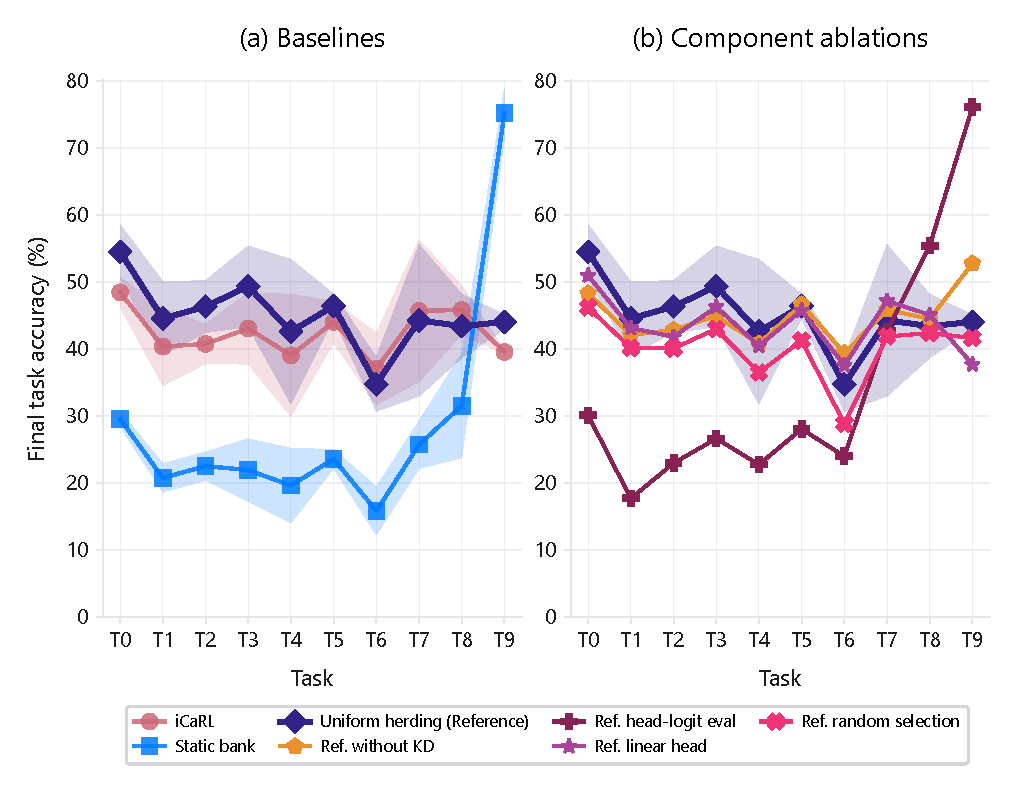
\includegraphics[width=\linewidth]{data/main/figures/fig1_per_task_accuracy.pdf}
  \caption{Final per-task accuracies. Panel (a) compares the baselines with
  Uniform Herding. Panel (b) shows the within-method variants. Shaded bands
  denote population standard deviation over three seeds.}
  \label{fig:per-task-accuracy}
\end{figure}

\subsection{Supporting Analyses of Uniform Herding}
\label{subsec:supporting-analyses}

Table~\ref{tab:t2-component-ablations} reports matched within-method changes
to the prediction rule, selection rule, distillation, and classifier head.
Replacing NME with head-logit evaluation reduces accuracy by $10.38$ pp and
increases forgetting by $32.50$ pp.  Replacing herding with random selection
reduces accuracy by $4.83$ pp and increases forgetting by $4.50$ pp.  Removing
KD changes accuracy by $-0.21$ pp but increases forgetting by $10.93$ pp,
whereas replacing the cosine-margin head with a linear head changes accuracy
by $-1.42$ pp and forgetting by $+0.83$ pp.  These are supporting comparisons
within the stated Uniform Herding protocol, not universal component effects.
Figure~\ref{fig:component-attribution} shows the matched per-seed changes.

\begin{table}[t]
  \centering
  \caption{Matched within-method comparisons for Uniform Herding. Deltas are
  paired by seed against the main configuration.}
  \label{tab:t2-component-ablations}
  \small
  \resizebox{\linewidth}{!}{%
  \begin{tabular}{lrrrr}
    \toprule
    Variant & Average accuracy (\%) & Forgetting (\%) & $\Delta$ accuracy (pp) & $\Delta$ forgetting (pp) \\
    \midrule
    Without KD & $44.79\pm0.31$ & $24.78\pm0.81$ & $-0.21$ & $+10.93$ \\
    Head-logit evaluation & $34.61\pm1.13$ & $46.36\pm1.63$ & $-10.38$ & $+32.50$ \\
    Linear head & $43.57\pm0.47$ & $14.68\pm0.48$ & $-1.42$ & $+0.83$ \\
    Random selection & $40.17\pm0.17$ & $18.35\pm0.61$ & $-4.83$ & $+4.50$ \\
    \bottomrule
  \end{tabular}
  }
\end{table}

\begin{figure}[t]
  \centering
  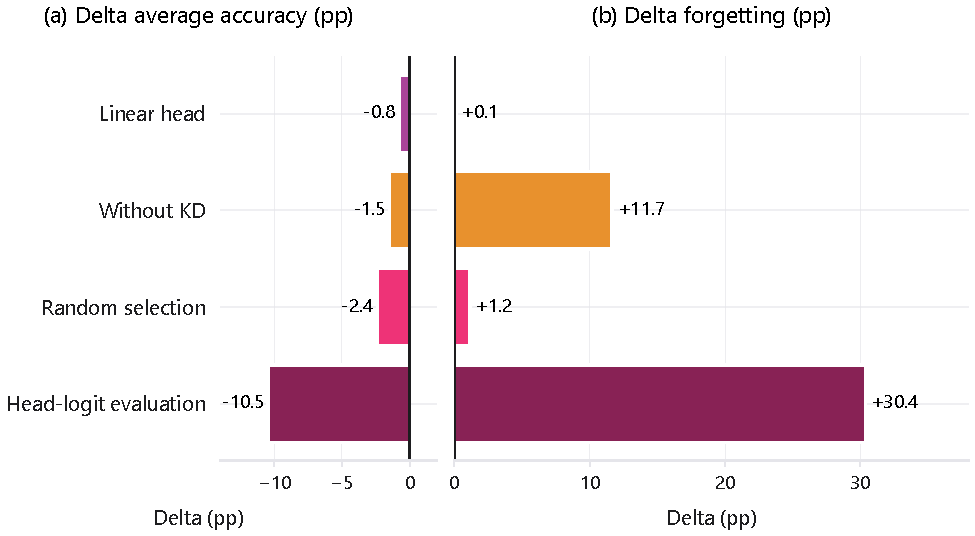
\includegraphics[width=\linewidth]{data/main/figures/fig2_component_attribution.pdf}
  \caption{Matched per-seed changes relative to Uniform Herding. Negative
  accuracy changes and positive forgetting changes are unfavorable.}
  \label{fig:component-attribution}
\end{figure}

\subsection{Active-Budget and Retrieval Sensitivity}
\label{subsec:resource-sensitivity}

Varying the active budget also changes the candidate-pool capacity because
Uniform Herding uses $\rho=3$.  Reducing $M$ from 2,000 to 500 lowers accuracy
by $8.17$ pp and raises forgetting by $5.77$ pp.  Increasing $M$ to 4,000
raises accuracy by $2.66$ pp and lowers forgetting by $1.18$ pp.  These three
points describe a tested-range resource pattern, not a scaling law.

With $M=2{,}000$ fixed, reducing retrieval from 64 to 32 changes accuracy by
$-1.71$ pp and forgetting by $+1.13$ pp.  Increasing retrieval to 128 changes
the corresponding means by $-0.18$ pp and $+0.81$ pp.  The retrieval sweep
therefore shows a smaller mean change over the tested values than the
active-budget sweep (Table~\ref{tab:t3-resource-sensitivity}).
Figure~\ref{fig:resource-sensitivity} visualizes these tested changes.

\begin{table}[t]
  \centering
  \caption{Resource sensitivity relative to Uniform Herding at $M=2{,}000$ and
  retrieval budget 64. Active-budget changes also change the candidate-pool
  capacity through $\rho=3$; deltas are paired by seed.}
  \label{tab:t3-resource-sensitivity}
  \small
  \resizebox{\linewidth}{!}{%
  \begin{tabular}{llrrrr}
    \toprule
    Axis & Value & Average accuracy (\%) & Forgetting (\%) & $\Delta$ accuracy (pp) & $\Delta$ forgetting (pp) \\
    \midrule
    Active budget & 500 & $36.83\pm0.36$ & $19.63\pm1.01$ & $-8.17$ & $+5.77$ \\
    Active budget & 2,000 & $44.99\pm1.00$ & $13.85\pm0.44$ & $0.00$ & $0.00$ \\
    Active budget & 4,000 & $47.66\pm0.72$ & $12.67\pm1.03$ & $+2.66$ & $-1.18$ \\
    Retrieval & 32 & $43.28\pm0.61$ & $14.98\pm0.99$ & $-1.71$ & $+1.13$ \\
    Retrieval & 64 & $44.99\pm1.00$ & $13.85\pm0.44$ & $0.00$ & $0.00$ \\
    Retrieval & 128 & $44.81\pm0.78$ & $14.66\pm0.75$ & $-0.18$ & $+0.81$ \\
    \bottomrule
  \end{tabular}
  }
\end{table}

\begin{figure}[t]
  \centering
  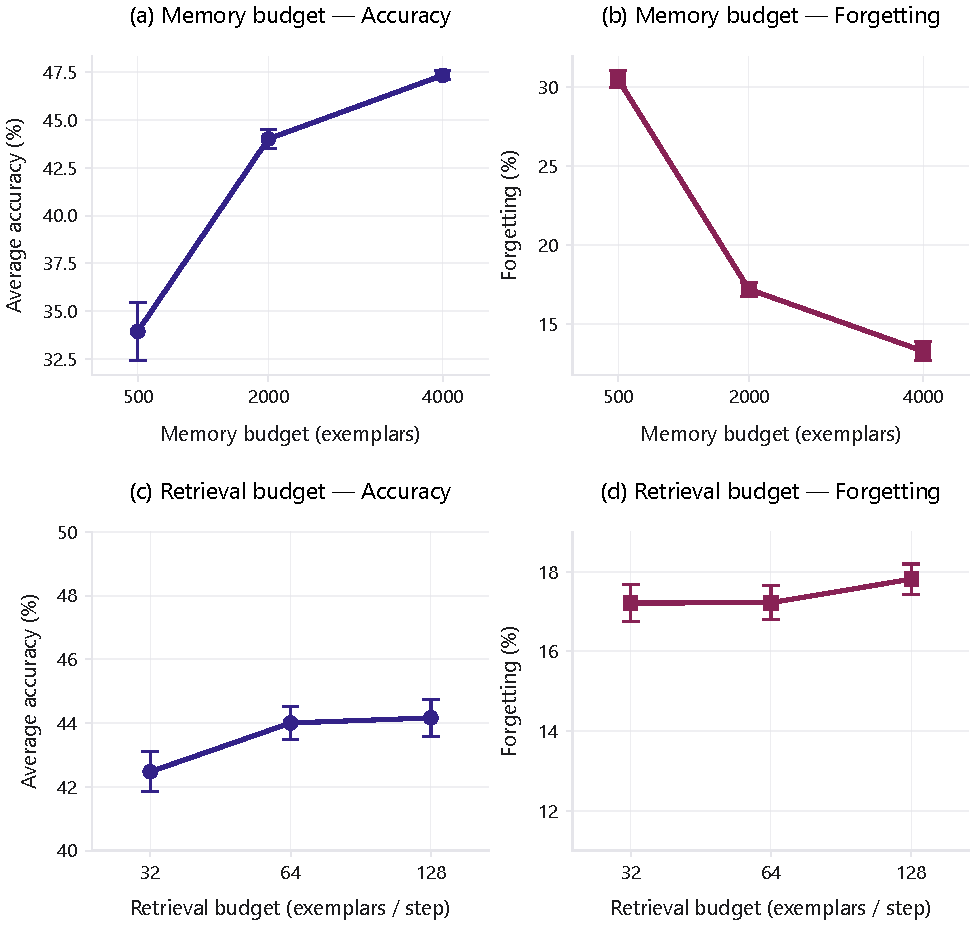
\includegraphics[width=\linewidth]{data/main/figures/fig3_resource_sensitivity.pdf}
  \caption{Sensitivity to active exemplar budget and replay retrieval budget.
  Error bars denote population standard deviation over three seeds.}
  \label{fig:resource-sensitivity}
\end{figure}

\subsection{Accuracy--Forgetting Trade-off}
\label{subsec:accuracy-forgetting-tradeoff}

Figure~\ref{fig:accuracy-forgetting} places the reported configurations in
the accuracy--forgetting plane.  At the common nominal active budget, Uniform
Herding has the highest mean accuracy and lowest mean forgetting among the
three main methods.  The plot is descriptive: its points vary method choices
and resource settings, so they do not define a single causal trade-off curve.

\begin{figure}[t]
  \centering
  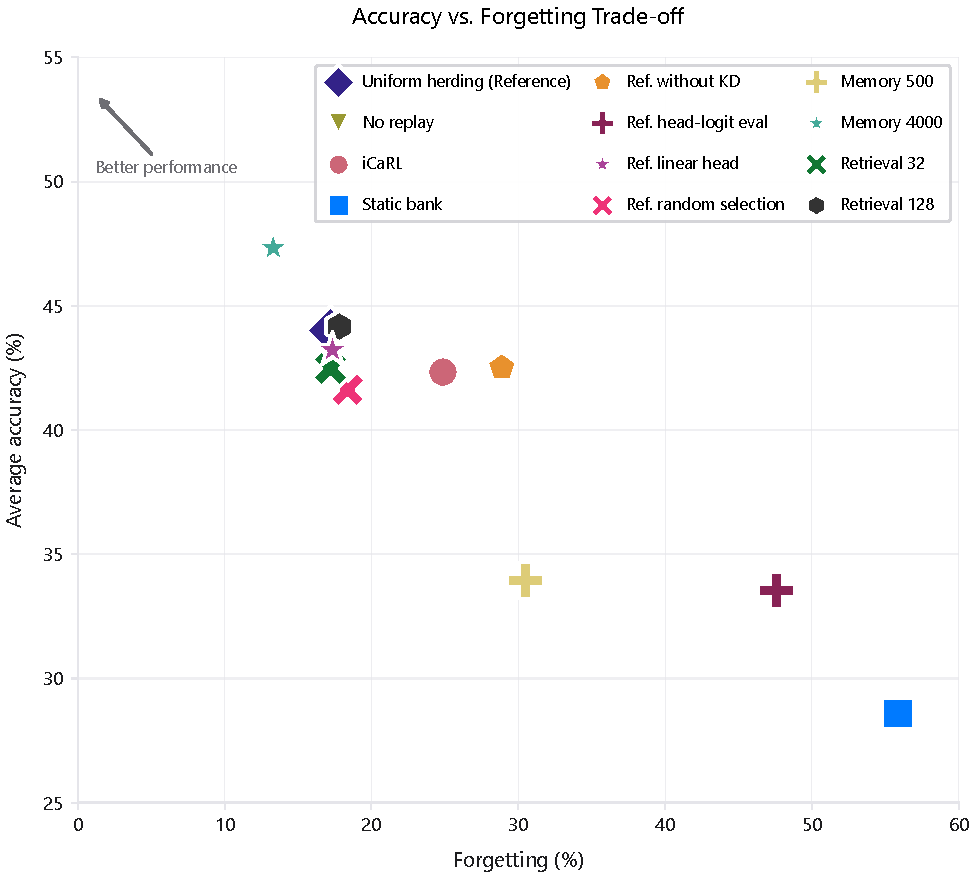
\includegraphics[width=0.92\linewidth]{data/main/figures/fig4_acc_forgetting_scatter.pdf}
  \caption{Average accuracy versus forgetting for baselines, within-method
  variants, and resource configurations. Higher accuracy and lower forgetting
  are preferred.}
  \label{fig:accuracy-forgetting}
\end{figure}

\subsection{Task-Age Failure Modes}
\label{subsec:task-age-failure-modes}

Figure~\ref{fig:forgetting-by-age} shows two contrasting failure modes.  The
static bank incurs approximately $51$--$59$ pp forgetting for tasks 0--8,
whereas head-logit evaluation incurs approximately $25$--$55$ pp.  Uniform
Herding ranges from $7.6$ to $26.8$ pp over these tasks.  In both adverse
configurations, the newest task has higher final accuracy than older tasks,
so aggregate accuracy can conceal recency bias.

The zero forgetting value for task 9 is structural: no later task can reduce
its accuracy under the final-task definition.  It is not evidence that the
last task is retained better than the preceding tasks.

\begin{figure}[t]
  \centering
  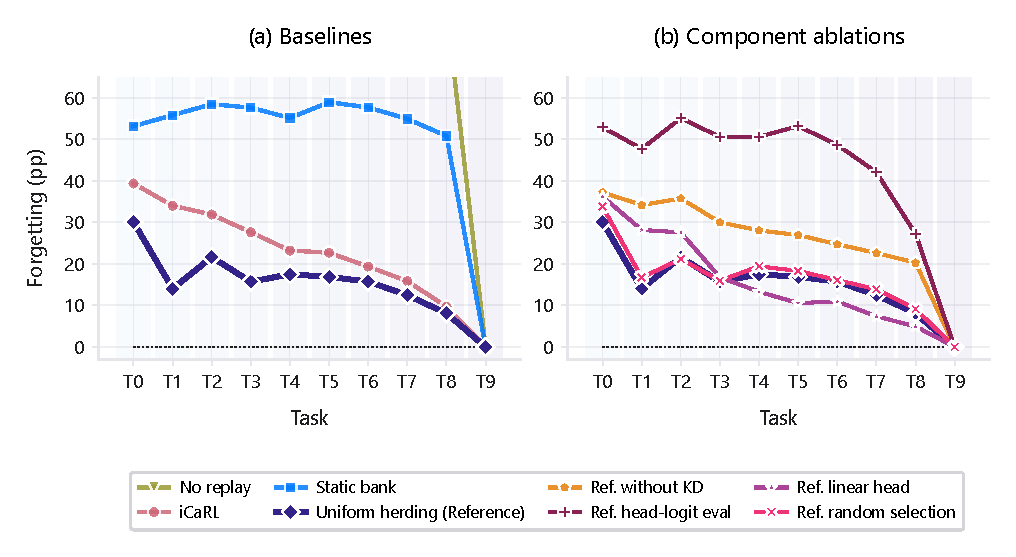
\includegraphics[width=\linewidth]{data/main/figures/fig5_forgetting_by_age.pdf}
  \caption{Forgetting by task index for Uniform Herding and two adverse
  configurations. The final task has zero forgetting by definition because no
  subsequent task is learned.}
  \label{fig:forgetting-by-age}
\end{figure}

\section{Discussion}
\label{sec:discussion}

The matched comparisons yield three practical findings: the prediction rule
produces the largest observed component difference, KD primarily affects
retention, and total exemplar memory has a larger observed effect than the
tested retrieval range.

\subsection{What Drives Performance}
\label{subsec:what-drives-performance}

We find that the final prediction rule is the largest measured lever in this
protocol. Replacing nearest-mean exemplar (NME) prediction with head-logit
prediction reduces final average accuracy by $10.38$ pp and increases
forgetting by $32.50$ pp (Table~\ref{tab:t2-component-ablations}). Both variants
use the same training procedure and differ only at prediction time; under this
comparison, head-logit prediction underperforms the selected-exemplar prototypes
used by NME.

KD has a distinct role. Removing it changes average accuracy by $-0.21$ pp
but raises forgetting by $10.93$ pp, consistent with KD acting as a retention
mechanism. Herding also matters once budget and replay procedure are held
fixed: replacing it with random selection reduces average accuracy by $4.83$
pp and increases forgetting by $4.50$ pp. By contrast, changing the training
head from cosine-margin to linear under NME prediction produces smaller
observed changes ($-1.42$ pp accuracy and $+0.83$ pp forgetting). Within this
protocol, prediction and exemplar selection therefore deserve priority over
head geometry when the objective is to improve the accuracy--forgetting trade-off.

\subsection{Resource Allocation and Design Implications}
\label{subsec:resource-allocation}

The resource sweep shows that storage matters more than retrieval count in the
tested range. Reducing memory from 2,000 to 500 exemplars loses $8.17$ pp in
accuracy and adds $5.77$ pp of forgetting. Doubling memory from 2,000 to
4,000 improves both metrics, whereas doubling retrieval from 64 to 128 does
not improve either mean metric (Table~\ref{tab:t3-resource-sensitivity}).
Retrieval may still matter, but expanding storage is the higher-priority
allocation in this setting.

For the evaluated setting, a replay system should allocate memory across all
observed classes, rebuild exemplars with herding, train with KD, and use NME
prediction. When additional resources are available, the measurements favor
expanding stored memory before increasing retrieval from 64 samples.

\subsection{Limitations}
\label{subsec:limitations}

Our claims are bounded by the protocol's coverage. All experiments use
CIFAR-100, one 10-task class partition induced by split seed 13, and a
ResNet-18 backbone. The three seeds quantify training variation but do not
measure sensitivity to alternative class orders, datasets, architectures, or
task granularities. The paired comparisons are based on three matched seeds;
they support the reported directions and magnitudes but do not provide
high-power estimates of small effects.

The memory sweep covers 500, 2,000, and 4,000 exemplars. Although the increase
from 2,000 to 4,000 is smaller than the loss from 2,000 to 500, these three
points do not establish a saturation threshold or a scaling law. The baseline
comparison isolates replay, selection, and prediction choices under a common
protocol. Extending the same matched ablations across class orders and standard
benchmarks is necessary to test whether the observed component ranking transfers.

\section{Conclusion}
\label{sec:conclusion}

This study examined how replay-system choices interact under a fixed-total
exemplar budget for CIFAR-100 class-incremental learning.  Holding the protocol
and resource budget fixed made it possible to separate exemplar selection,
distillation, classifier head, and evaluation readout.  The matched ablations
show that nearest-mean exemplar evaluation and herding are the largest measured
contributors to the reference configuration's accuracy--forgetting trade-off.
Distillation primarily improves retention, whereas the memory sweep has a
larger effect than the tested changes in retrieval budget.

For the measured setting, a defensible replay design is to allocate memory
across all observed classes, rebuild representative exemplars in the current
feature space, train with distillation, and evaluate with the corresponding NME
prototypes.  This is a protocol-specific recommendation, not a general ranking
of class-incremental methods.  The next empirical step is to test the same
component-level analysis across class orders, datasets, architectures, and
larger memory ranges.


\bibliographystyle{plain}
\bibliography{bib/references}

\clearpage
\appendix
\section{Reproducibility Details}
\label{app:reproducibility}

All experiments used CIFAR-100 in a fixed ten-task class-incremental
partition of ten classes per task. The class partition was determined by split
seed 13 and was shared by all runs; the three reported seeds therefore vary
training randomness rather than class order. Each task was trained with a
ResNet-18 (64 base filters, no dropout), batch size 128, mixed-precision
arithmetic, and SGD with learning rate 0.1, momentum 0.9, weight decay
$5\times10^{-4}$, and gradient clipping at 1.0. No learning-rate schedule or
warm-up was used. The configured task length was 70 epochs. Run metadata
records 71 epochs for every seed because the trainer's epoch counter was
incremented once after the final configured epoch; this recording discrepancy
does not alter the configured schedule.

Unless an ablation changes the relevant component, models use the cosine-margin
head (scale 30, margin 0.35) with weight imprinting of each new task's head rows
(after task 0, which retains its random initialization), a distillation weight
of 1 at temperature 2, and a retrieval budget of 64. The no-distillation
ablation sets the distillation weight to zero; the linear-head ablation replaces
the cosine-margin head. The static-bank baseline and the head-logit evaluation
ablation use head-logit prediction; all other reported configurations use NME
prediction. Table~\ref{tab:app-protocol} gives the remaining protocol settings.

\begin{table}[t]
  \centering
  \caption{Protocol settings shared across runs unless an ablation explicitly
  changes them.}
  \label{tab:app-protocol}
  \small
  \resizebox{\linewidth}{!}{%
  \begin{tabular}{ll}
    \toprule
    Setting & Value \\
    \midrule
    Dataset and partition & CIFAR-100; 10 tasks $\times$ 10 classes; split seed 13 \\
    Probe / validation split & 30 / 20 \\
    Backbone & ResNet-18; 64 base filters; dropout 0 \\
    Optimizer & SGD; lr 0.1; momentum 0.9; weight decay $5\times10^{-4}$ \\
    Training & 70 configured epochs per task; batch size 128; gradient clip 1.0 \\
    Precision & 16-mixed \\
    Random seeds & 1993, 2023, 42 \\
    Default exemplar budget & 2,000 \\
    Default retrieval budget & 64 \\
    Hardware & Tesla T4 \\
    Software & Python 3.12.13; PyTorch 2.11.0+cu128; Lightning 2.6.5 \\
    \bottomrule
  \end{tabular}
  }
\end{table}

\section{Task-Level Results}
\label{app:task-results}

For task $i$, the reported forgetting is the difference between the best
accuracy attained on task $i$ during training and its accuracy after the final
task. Figure~\ref{fig:app-forgetting} gives this quantity for every method and
task. The final task has zero forgetting by construction. The figure therefore
separates aggregate retention from its distribution over task age and avoids
inferring a trajectory from a single summary statistic.

\begin{figure}[t]
  \centering
  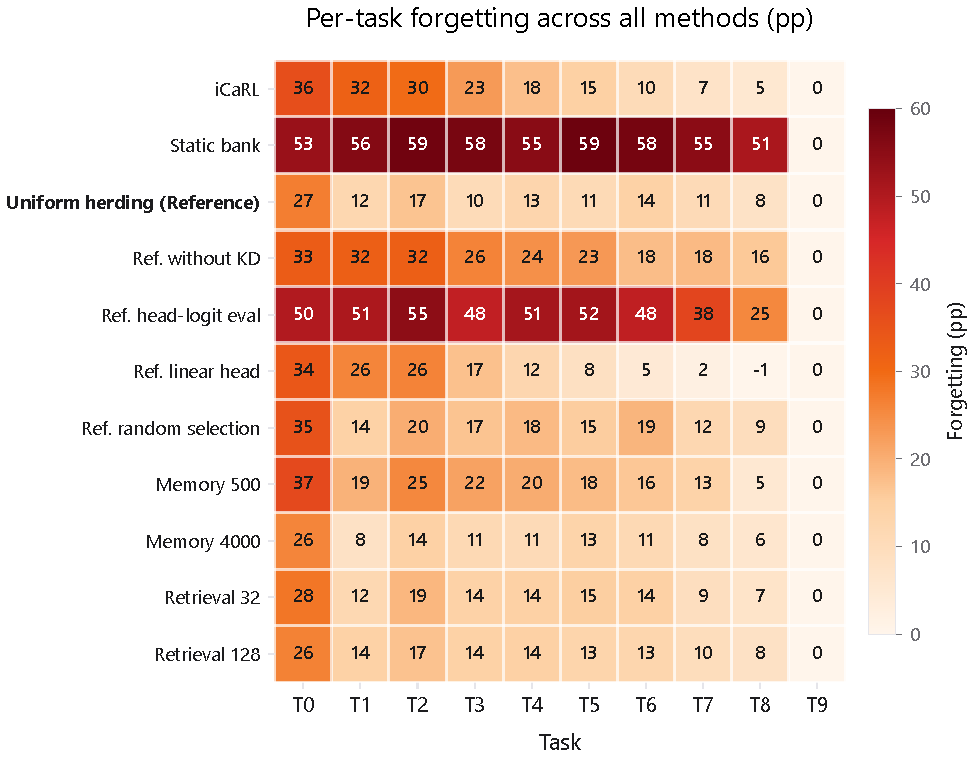
\includegraphics[width=\linewidth]{data/appendix/figures/figA1_forgetting_heatmap.pdf}
  \caption{Per-task forgetting, in percentage points, for all evaluated
  configurations. Each entry is the drop from the task's best observed accuracy
  to its final accuracy. Task T9 is zero by definition because it is introduced
  last.}
  \label{fig:app-forgetting}
\end{figure}

Figures~\ref{fig:app-reference-evolution} and~\ref{fig:app-icarl-evolution}
show the complete task-by-time accuracy matrices for the reference method and
iCaRL, respectively. Row $i$, column $t$ is the accuracy on task $i$ after
learning through task $t$; cells with $i>t$ are undefined and omitted. These
matrices are the underlying trajectories from which the task-level forgetting
values are calculated.

\begin{figure}[t]
  \centering
  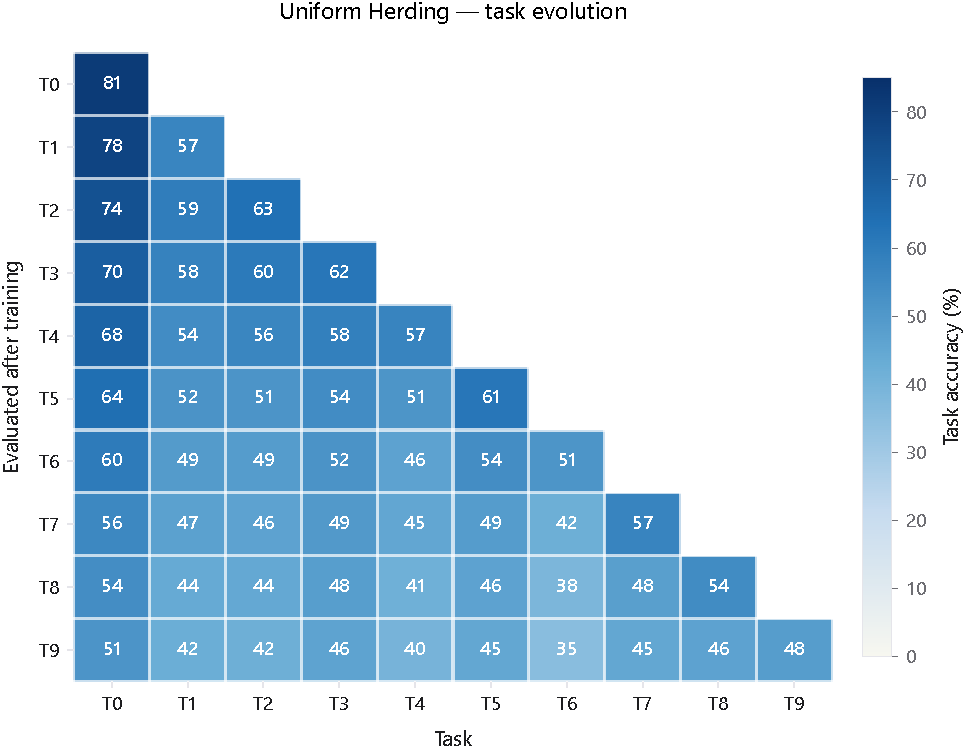
\includegraphics[width=\linewidth]{data/appendix/figures/figA2_evolution_reference.pdf}
  \caption{Task-evolution accuracy matrix for uniform herding with NME
  prediction (the reference configuration).}
  \label{fig:app-reference-evolution}
\end{figure}

\begin{figure}[t]
  \centering
  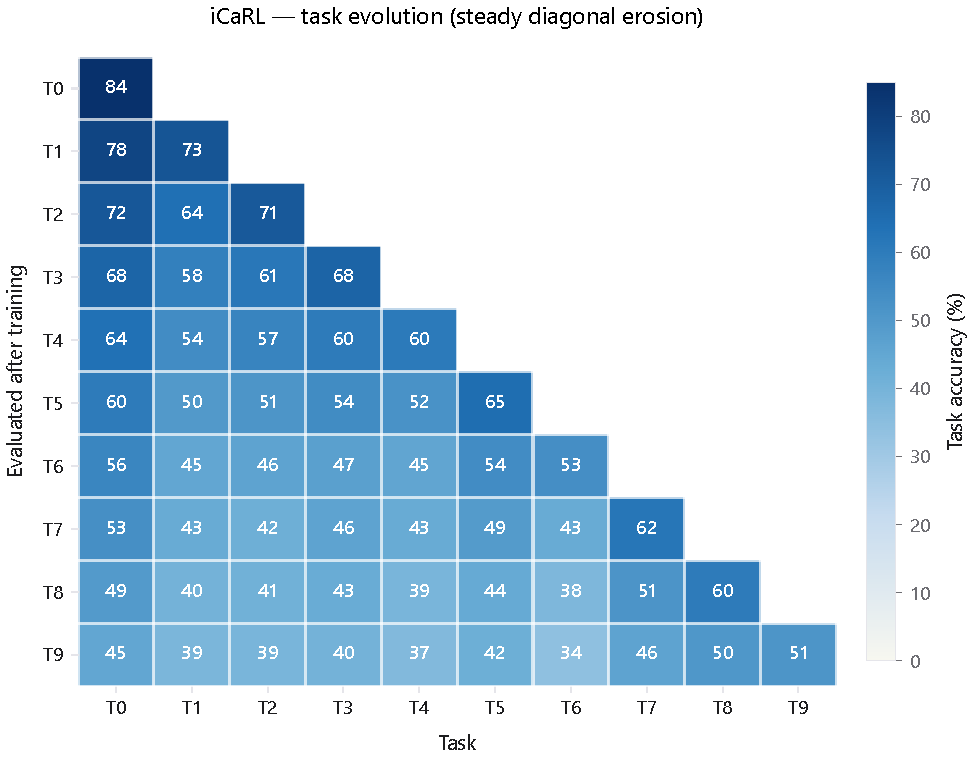
\includegraphics[width=\linewidth]{data/appendix/figures/figA3_evolution_icarl.pdf}
  \caption{Task-evolution accuracy matrix for iCaRL.}
  \label{fig:app-icarl-evolution}
\end{figure}

Figure~\ref{fig:app-kd-slopes} provides a seed-level view of the principal
stability comparison. For each earlier task and each seed, it connects the
accuracy at introduction with the final accuracy. It is a visualization of the
same per-seed measurements summarized in the main text, not an additional
statistical test.

\begin{figure}[t]
  \centering
  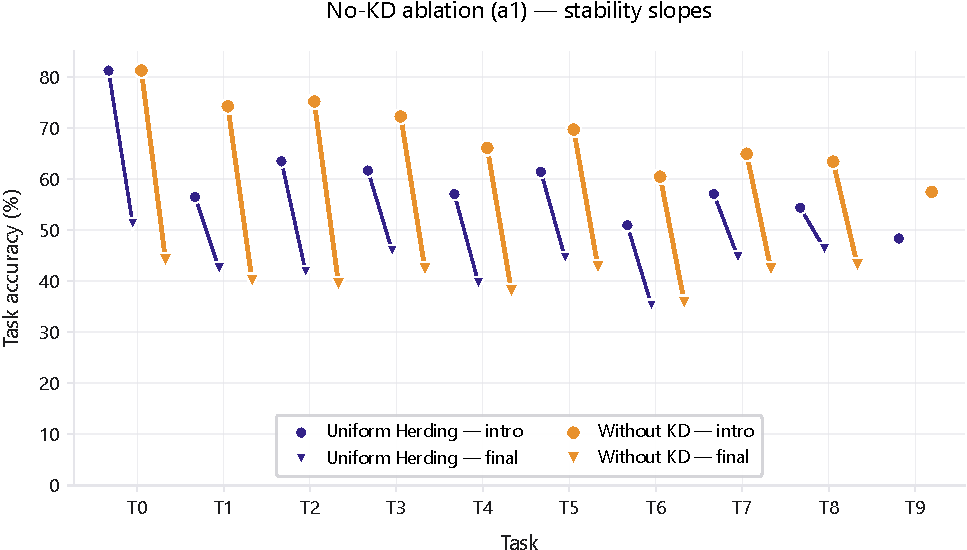
\includegraphics[width=\linewidth]{data/appendix/figures/figA4_stability_slopes.pdf}
  \caption{Seed-level task trajectories for the reference configuration and the
  no-distillation ablation. Lines connect task-introduction accuracy to final
  accuracy for the same task and seed.}
  \label{fig:app-kd-slopes}
\end{figure}

\section{Seed-Level Outcomes and Compute}
\label{app:seed-compute}

Table~\ref{tab:app-seeds} reports the raw aggregate metrics for every run and
seed. Values are percentages. This table is included to make the means and
standard deviations in the main text auditable without treating the three
training seeds as independent task-level observations.

\begin{table}[t]
  \centering
  \caption{Per-seed final average accuracy, forgetting, and backward transfer.}
  \label{tab:app-seeds}
  \scriptsize
  \begin{tabular}{llrrr}
    \toprule
    ID & Configuration / seed & Average accuracy & Forgetting & BWT \\
    \midrule
    B1 & iCaRL / 1993 & 42.29 & 19.50 & -19.50 \\
    B1 & iCaRL / 2023 & 43.46 & 19.32 & -19.32 \\
    B1 & iCaRL / 42 & 41.33 & 19.56 & -19.56 \\
    B2 & Static bank / 1993 & 28.15 & 56.34 & -56.34 \\
    B2 & Static bank / 2023 & 30.43 & 53.93 & -53.93 \\
    B2 & Static bank / 42 & 27.22 & 57.31 & -57.31 \\
    B3 & Reference / 1993 & 45.11 & 13.37 & -13.17 \\
    B3 & Reference / 2023 & 46.16 & 13.77 & -13.38 \\
    B3 & Reference / 42 & 43.71 & 14.42 & -14.09 \\
    a1 & No KD / 1993 & 45.22 & 23.68 & -23.68 \\
    a1 & No KD / 2023 & 44.54 & 25.07 & -25.07 \\
    a1 & No KD / 42 & 44.60 & 25.59 & -25.59 \\
    a2 & Head-logit / 1993 & 33.09 & 48.07 & -48.07 \\
    a2 & Head-logit / 2023 & 34.93 & 46.83 & -46.83 \\
    a2 & Head-logit / 42 & 35.81 & 44.17 & -44.17 \\
    a3 & Linear head / 1993 & 43.77 & 15.07 & -14.70 \\
    a3 & Linear head / 2023 & 44.02 & 14.97 & -14.82 \\
    a3 & Linear head / 42 & 42.92 & 14.00 & -13.50 \\
    a4 & Random selection / 1993 & 39.94 & 18.31 & -17.90 \\
    a4 & Random selection / 2023 & 40.35 & 19.11 & -18.20 \\
    a4 & Random selection / 42 & 40.21 & 17.62 & -17.16 \\
    s1 & Memory 500 / 1993 & 36.64 & 18.24 & -18.24 \\
    s1 & Memory 500 / 2023 & 37.33 & 20.61 & -20.61 \\
    s1 & Memory 500 / 42 & 36.51 & 20.02 & -20.02 \\
    s2 & Memory 4000 / 1993 & 47.60 & 11.40 & -10.93 \\
    s2 & Memory 4000 / 2023 & 48.56 & 12.68 & -12.33 \\
    s2 & Memory 4000 / 42 & 46.81 & 13.93 & -13.10 \\
    s3 & Retrieval 32 / 1993 & 43.46 & 13.99 & -13.92 \\
    s3 & Retrieval 32 / 2023 & 43.92 & 16.33 & -15.86 \\
    s3 & Retrieval 32 / 42 & 42.46 & 14.62 & -14.24 \\
    s4 & Retrieval 128 / 1993 & 44.57 & 13.62 & -13.52 \\
    s4 & Retrieval 128 / 2023 & 45.86 & 15.03 & -14.66 \\
    s4 & Retrieval 128 / 42 & 44.00 & 15.33 & -14.96 \\
    \bottomrule
  \end{tabular}
\end{table}

Table~\ref{tab:app-compute} reports elapsed wall-clock time per run on a Tesla
T4. These timings describe the implementation and hardware used here; they are
not intended as hardware-independent efficiency comparisons.

\begin{table}[t]
  \centering
  \caption{Wall-clock time per run in seconds (mean $\pm$ standard deviation
  across the three seeds), measured on a Tesla T4.}
  \label{tab:app-compute}
  \small
  \begin{tabular}{llr}
    \toprule
    ID & Configuration & Seconds \\
    \midrule
    B1 & iCaRL & $3754.8 \pm 38.0$ \\
    B2 & Static bank & $2716.3 \pm 91.6$ \\
    B3 & Reference & $4493.2 \pm 52.5$ \\
    a1 & No KD & $3307.7 \pm 54.0$ \\
    a2 & Head-logit & $4279.5 \pm 93.4$ \\
    a3 & Linear head & $3732.1 \pm 42.7$ \\
    a4 & Random selection & $4555.9 \pm 37.1$ \\
    s1 & Memory 500 & $4292.4 \pm 54.2$ \\
    s2 & Memory 4000 & $4351.7 \pm 26.0$ \\
    s3 & Retrieval 32 & $3958.1 \pm 104.2$ \\
    s4 & Retrieval 128 & $5919.2 \pm 49.9$ \\
    \bottomrule
  \end{tabular}
\end{table}

\section{Exemplar Quotas}
\label{app:quotas}

After task $t$, the available memory is divided among the $10(t+1)$ observed
classes. Table~\ref{tab:app-quotas} lists the resulting per-class quotas. When
the budget is not divisible by the number of observed classes, the allocation
uses floor rounding and adjacent classes can differ by one exemplar.

\begin{table}[t]
  \centering
  \caption{Per-class exemplar quota after each task. Ranges indicate the
  one-exemplar difference induced by floor rounding.}
  \label{tab:app-quotas}
  \small
  \resizebox{\linewidth}{!}{%
  \begin{tabular}{lrrrrrrrrrr}
    \toprule
    Budget & T0 & T1 & T2 & T3 & T4 & T5 & T6 & T7 & T8 & T9 \\
    \midrule
    500 & 50 & 25 & 16--17 & 12--13 & 10 & 8--9 & 7--8 & 6--7 & 5--6 & 5 \\
    2,000 & 200 & 100 & 66--67 & 50 & 40 & 33--34 & 28--29 & 25 & 22--23 & 20 \\
    4,000 & 400 & 200 & 133--134 & 100 & 80 & 66--67 & 57--58 & 50 & 44--45 & 40 \\
    \bottomrule
  \end{tabular}
  }
\end{table}


\end{document}
